% LaTeX.tex
% Example of PROCEEDINGS PAPER of the 26th ABCM International Congress of Mechanical Engineering
% COBEM 2021 - ONLINE
% Based on the templates of COBEM2015, COBEM2017, and COBEM2019

\documentclass[10pt,fleqn,a4paper,twoside]{article}
\usepackage{abcm}
\def\shortauthor{F. Author, S. Author and T. Author (update this heading accordingly)}
\def\shorttitle{Paper Short Title (First Letters Uppercase, make sure it fits in one line)}

\begin{document}
\fphead
\hspace*{-2.5mm}\begin{tabular}{||p{\textwidth}}
\begin{center}
\vspace{-4mm}
\title{COB-2021-XXXX {\color{red}(XXXX is the identification number of the final paper)}\\
INSTRUCTIONS FOR FORMATTING THE PROCEEDINGS PAPERS OF THE 26$^{\mathrm{th}}$ COBEM}
\end{center}
\authors{First Author's Name} \\
\authors{Second Author's Name} \\
\institution{Institution and address for first and second authors - if the same} \\
\institution{e-mails} \\
\\
\authors{Third Author's Name} \\
\institution{Institution and address for third author} \\ %(If all authors are from the same institution, the "Institution and address" must be placed only once.)
\institution{e-mail} \\
\\
\authors{Same format for others authors, if any} \\
\\
\abstract{\textbf{Abstract.} The abstract should describe the objectives, the context and importance of the research, the methods, the results and the main conclusions of the paper in about 200 words. It should not contain neither formulae nor reference to bibliography. It must be written in only one paragraph.}\\
\\
\keywords{\textbf{Keywords:} keyword 1, keyword 2, keyword 3, \dots{}. (up to 5 keywords, separated with commas)}\\
\end{tabular}

\section{INTRODUCTION}

The purpose of these instructions is to serve as a guide for formatting the {\bf papers} to be published in the proceedings. The proceedings of the 26$^{\mathrm{th}}$ COBEM will be published in Adobe\texttrademark\space PDF format.

The proceedings papers {\bf MUST} be formatted according to these instructions. The present file can be used as a template for \LaTeX\space users. Also, it could be used as a formatting guide to users of other word processors.

The papers are limited to a minimum of {\bf 6} pages and a maximum of {\bf 10} pages, including tables and figures. 

\section{TEXT FORMAT}

The manuscripts should be written in English, typed in A4 size pages, using font Times New Roman, size 10, except for the title, authors affiliation, abstract and keywords, for which particular formatting instructions are indicated above. Single space between lines is to be used throughout the text.

The text block that contains the title, the authors' names and affiliation, the abstract and the keywords must be indented 0.1 cm from the left margin and marked by a leftmost black line border of width 2 1/4 pt.

The first page must have a top margin of 3 cm and all the other margins (left, right and bottom) must have 2 cm. The body of the text must be justified. The first line of each paragraph must be indented by 0.5 cm. Sufficient information must be provided directly in the text, or by reference to widely available published work. Footnotes should be avoided. 

{\color{red} PAGES {\bf SHOULD NOT} BE NUMBERED.}

All the symbols and notation must be defined in the text. Physical quantities must be expressed in the SI (metric) units. Mathematical symbols appearing in the text must be typed in italic style. Units must be typed in roman style (e.g., kg, m, MJ, kW/m$^2$, \dots, instead of $kg$, $m$, $MJ$, $kW / m^2$, \dots). 

Bibliographic references should be cited in the text by giving the last name of the author(s) and the year of publication, according to the following examples: ``Recent work~\citep{Simas2019}\dots'' or ``Recently, \citet{Simas2019}\dots''. In the case of three or more authors, the form ``\citep{Bravo2018}'' should be used. Two or more references having the same authors and publication year must be distinguished by appending ``a'', ``b'', etc., to the year of publication. For example: ``In the works of~\citet{Santos2013a} and \citet{Santos2013b}, \dots''.

Acceptable references include journal articles~\citep{Bravo2018}, articles published in conference proceedings~\citep{Santos2013a}~\citep{Santos2013b}, conference proceedings~\citep{Carvalho2017}, books~\citep{MendoncaFancello2019}~, Master's Theses~\citep{Campos2018} and Doctoral Dissertations or Doctoral Theses~\citep{Grando2017}, patents~\citep{Fernandes2018}, reports, when publicly available,~\citep{EPE2020}, websites and specific pages in websites ~\citep{MLA20}, and submitted articles (if the journal is identified).

References should be listed at the end of the manuscript according to instructions provided in Section~\ref{Sec:references}.

\subsection{Section titles and subtitles}

The section titles and subtitles must be aligned at left, typed with Times New Roman, size 10, bold style font. They must be numbered using Arabic numerals separated by points. No more than 3 levels (\emph{section}, \emph{subsection}, and \emph{subsubsection}) should be used. 

A vertical space equivalent to one single line must be included above and bellow each section title/subtitle.

\subsection{Mathematical equations}

The mathematical equations must be indented by 0.5 cm from the left margin. They must be typed using Times New Roman, italic, size 10 pt. font. Arabic numerals must be used as equation numbers, enclosed between parentheses, right-aligned, as shown in the examples below. Equations should be referred to either as ``Eq.~(\ref{Eq:1})'' in the middle of a phrase or as ``Equation~(\ref{Eq:1})'' in the beginning of a sentence. Matrix and vector quantities can be indicated either by brackets and braces, as in Eq.~(\ref{Eq:1}), or in bold style, as in Eq.~(\ref{Eq:2}). Symbols used in the equations must be defined immediately before or after their first appearance. A vertical space equivalent to one blank line must be included above and below each equation.

``The equation of the dynamical system is written in one of the two forms,
\begin{equation}
[M]\{\ddot{x}\}+[C]\{\dot{x}(t)\}+[K]\{x(t)\}={f(t)},
\label{Eq:1}
\end{equation}
or,
\begin{equation}
\mathbf{M}\ \ddot{\mathbf{x}}(t)+\mathbf{C}\ \dot{\mathbf{x}}(t)+\mathbf{K}\ \mathbf{x}(t)=\mathbf{f}(t), 
\label{Eq:2}
\end{equation}
where $[M]$ or $\mathbf{M}$, $[C]$ or $\mathbf{C}$, and $[K]$ or $\mathbf{K}$ are the mass, dissipation and stiffness matrices, respectively, and $[\ddot{x}]$ or $\ddot{\mathbf{x}}$, $[\dot{x}]$ or $\dot{\mathbf{x}}$, $[x]$ or $\mathbf{x}$, and $[f]$ or $\mathbf{f}$ are the acceleration, velocity, displacement, and input force vectors, respectively.''

\subsection{Figures and tables}

Figures and tables should be placed in the text as close as possible to the point they are first mentioned and must be numbered consecutively in Arabic numerals. Figures must be referred to either as ``Fig.~\ref{Fig:1}'' in the middle of a phrase or as ``Figure~\ref{Fig:1}'' in the beginning of a sentence. The figures themselves as well as their captions must be centered in the breadth-wise direction. The captions of the figures should not be longer than 3 lines.

\begin{figure}[h!]
\centering
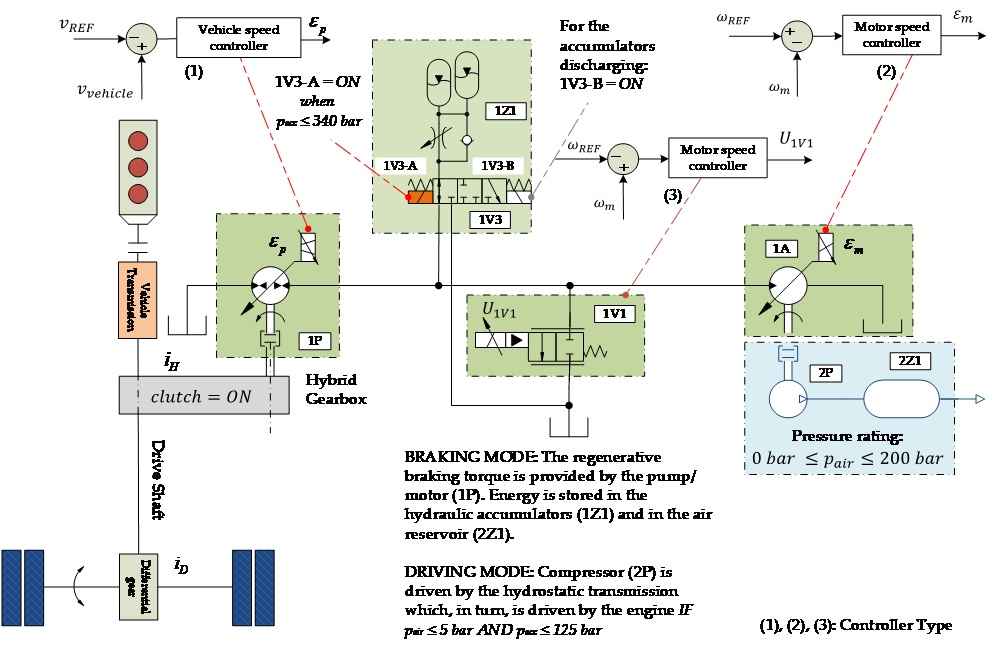
\includegraphics[angle=0, width=17cm]{figure.jpg}
\caption{Schematic diagram of the control strategy.}
\label{Fig:1}
\end{figure}

A vertical space equivalent to one single line must be left before and after each figure.

The legend for the data symbols as well as the labels for each curve should be included into the figure. Lettering should be large enough for ease reading. All units must be expressed in the S.I. (metric) system.

Color figures and high-quality photographs can be included in the manuscript. To reduce the file size and preserve the graphic resolution, figures must be saved into GIF (figures with less than 16 colors) or JPEG (for higher color density) files before being inserted in the manuscript.

Tables must be referred to either as ``Tab.~\ref{Tab:1}'' in the middle of a phrase or as ``Table~\ref{Tab:1}'' in the beginning of a sentence.  The tables themselves as well as their titles must be centered in the breadth-wise direction. The titles of the tables should not be longer than 3 lines. The font style and size used in the tables must be similar (both in size and style) to those used in the text body. Units must be expressed in the S.I. (metric) system. Explanations, if any, should be given at the foot of the tables, not within the tables themselves. The style of table borders is left free. An example is given in Tab.~\ref{Tab:1}.

A vertical space equivalent to one single line must be left before and after each table.

\begin{table}[!h]
\centering
\caption{Experimental results for flexural properties of CFRC-4HS and CFRC-TWILL composites. \protect\\Span/depth ratio = 35:1. Average results of 7 specimens.}
\label{Tab:1}
\begin{tabular}{l|c|c}
\hline
\textbf{Composite Properties} & \textbf{CFRC-TWILL} & \textbf{CFRC-4HS}\\
\hline
Flexural Strength\footnotesize{$^{(1)}$}, MPa & 209$\pm$ 10 & 180 $\pm$  15\\
Flexural Modulus\footnotesize{$^{(1)}$}, GPa & 57.0 $\pm$ 2.8 & 18.0 $\pm$  1.3\\
Mid-span deflection at the failure stress, mm & 2.15 $\pm$  1.90 & 6.40 $\pm$  0.25\\
\hline
\multicolumn{3}{l}{\footnotesize{$^{(1)}$ Measured at 25 $^{o}$C.}}
\end{tabular}
\end{table}

\section{ACKNOWLEDGEMENTS}
This optional section must be placed before the list of references.

\section{REFERENCES} 
\label{Sec:references}

The list of references must be introduced as a new section, located at the end of the manuscript. The first line of each reference must be aligned at left.  All the other lines must be indented by 0.5 cm from the left margin. All references included in the reference list must have been mentioned in the text.

References must be listed in alphabetical order, according to the last name of the first author. See the following examples:

\bibliographystyle{abcm}
\renewcommand{\refname}{}
\bibliography{bibfile}

\section{RESPONSIBILITY NOTICE}
The following text, properly adapted to the number of authors, must be included in the last section of the paper:

The author(s) is (are) solely responsible for the printed material included in this paper.

\end{document}
